\documentclass[11pt,compress,t,notes=noshow, aspectratio=169, xcolor=table]{beamer}
% deactivate beamer navigation
%\setbeamertemplate{navigation symbols}{}
%\usepackage{geometry}
%\geometry{papersize={180mm, 135mm}, top=-1.5mm} % 210mm, 297mm

\usepackage{multicol}
% set path of iml lecture here, e.g., relative to the current dir
\newcommand{\pathiml}{../}
\usepackage{\pathiml/style/lmu-lecture-bak}
\usepackage{pax}
\setbeamertemplate{frametitle}{\expandafter\uppercase\expandafter\insertframetitle}
%\useoutertheme{metropolis}
% remove section slides
\AtBeginSection[]
{
  \begin{frame}<beamer>
    \frametitle{Introduction to IML}
    %\begin{multicols}{2}
    \tableofcontents[currentsection]
    %\end{multicols}
  \end{frame}
}
% includepdf slides, pagecommad will set counter for framenumber
\usepackage{pdfpages}
\includepdfset{trim=0mm 0mm 42mm 0mm, pagecommand={\global\setcounter{framenumber}{\value{page}}}}
%trim=left bottom right top,clip
% trim=0mm 6mm 0mm 0mm, offset=0 15,
% add footer:
\usepackage{framed, color}
\usepackage{xcolor}
%\iffalse
\setbeamertemplate{footline}[text line]{%
    \noindent\hspace*{\dimexpr-\oddsidemargin-1in\relax}%
     \colorbox{white}{
     \makebox[\dimexpr\paperwidth-2\fboxsep\relax]{
     \color{black}
     \begin{minipage}[c][2ex][c]{0.5\linewidth}
       \secname
     \end{minipage}
     \hfill\begin{minipage}[c][2ex][c]{0.5\linewidth}
       \flushright
       \insertframenumber{}~/~\inserttotalframenumber~~
     \end{minipage}
     }}%
  \hspace*{-\paperwidth}
}
%\fi

\begin{document}
\setbeamercolor{background canvas}{bg=}

% General remark: hyperlinks in included pdfs are not clickable anymore in the combined pdf unless you use pax to extract annotations from original files and complile this file locally (see https://tex.stackexchange.com/questions/497624/merging-multiple-pdf-files-without-breaking-hyperlinks)

\section{Introduction, Motivation and History}
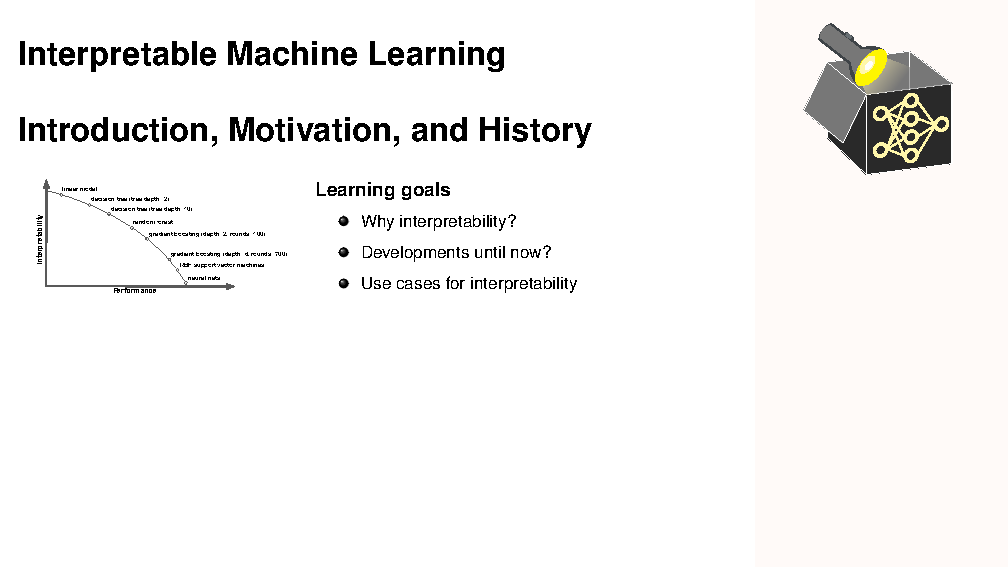
\includepdf[pages={1, 3-last}]{slides01-intro-motivation.pdf}
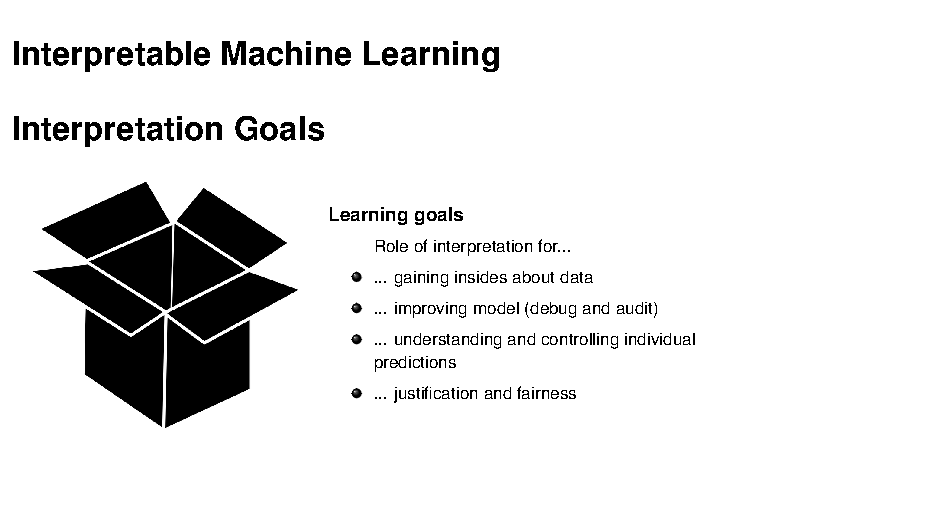
\includepdf[pages={1-4, 6, 8-13}]{slides02-intro-goals.pdf}
\includepdf[pages={1-13}]{slides03-intro-dimensions.pdf}
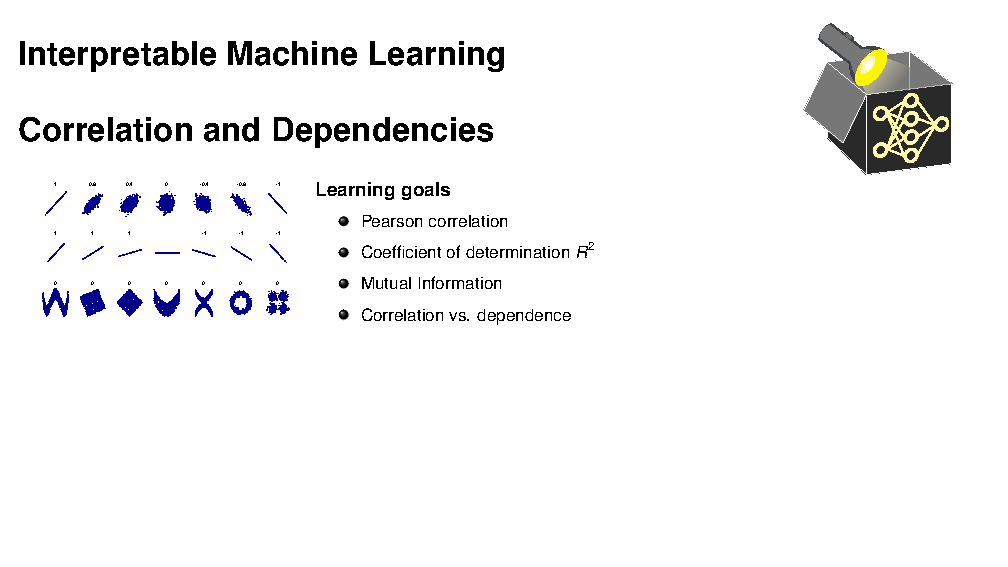
\includepdf[pages={1-3, 10-11, 18, 13, last}]{slides04-intro-correlation.pdf}
\includepdf[pages={9-12}]{slides06-intro-pitfalls.pdf}
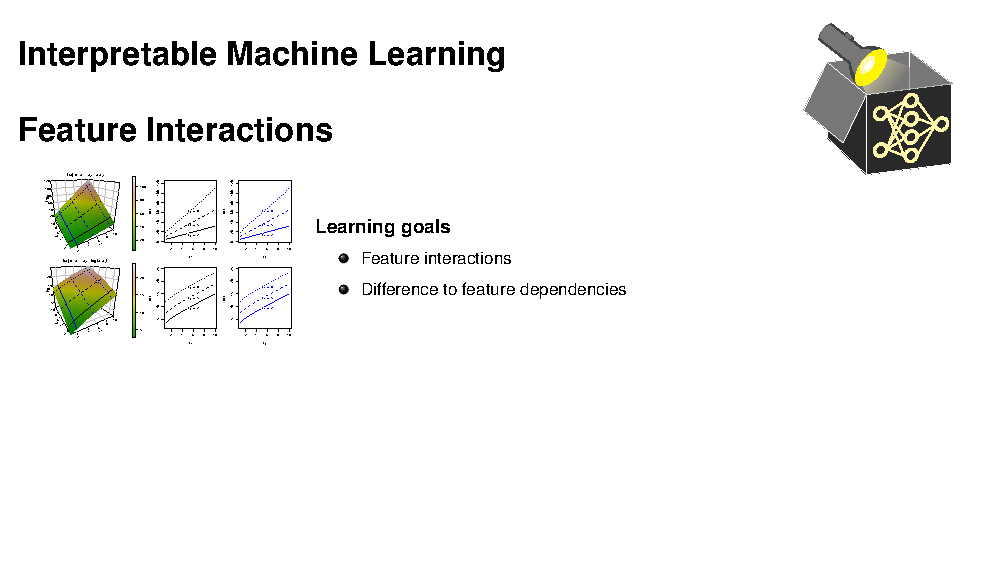
\includepdf[pages={1-last}]{slides05-intro-interaction.pdf}
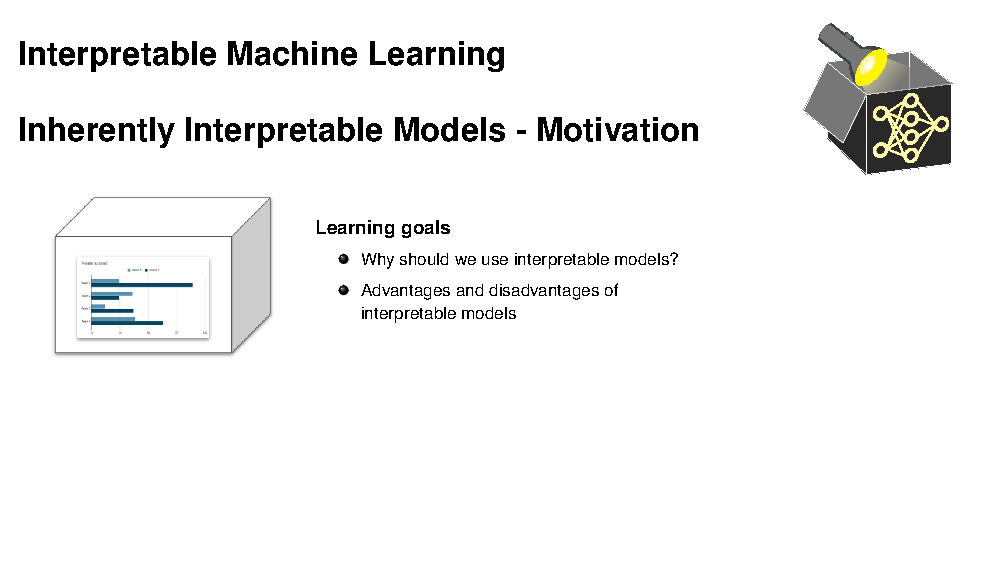
\includepdf[pages={1-last}]{slides01-im-motivation.pdf}

\section{Feature Effects - ICE and PDP}
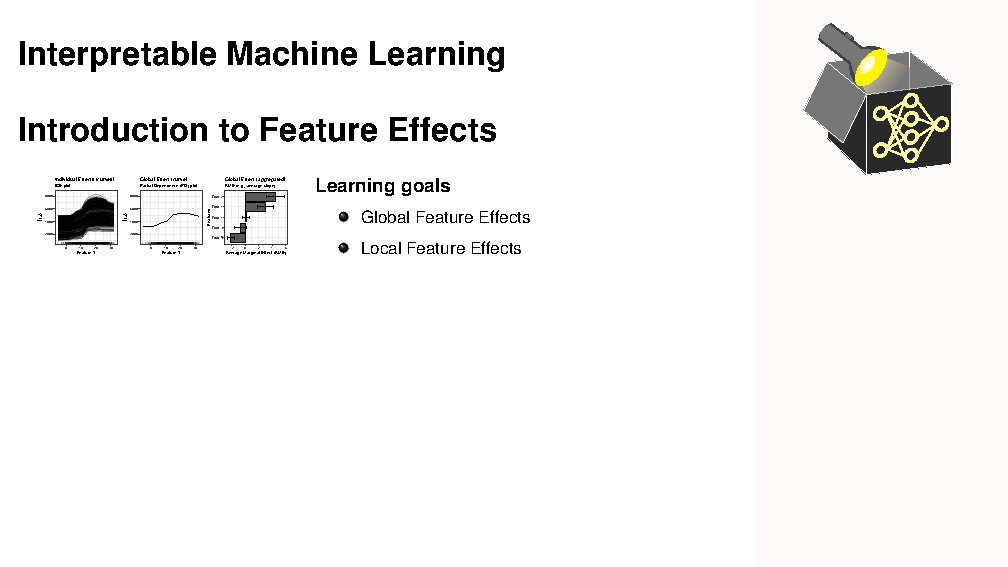
\includepdf[pages={1-6}]{slides01-fe-intro.pdf}
%\section{Feature Effects - ICE curves}
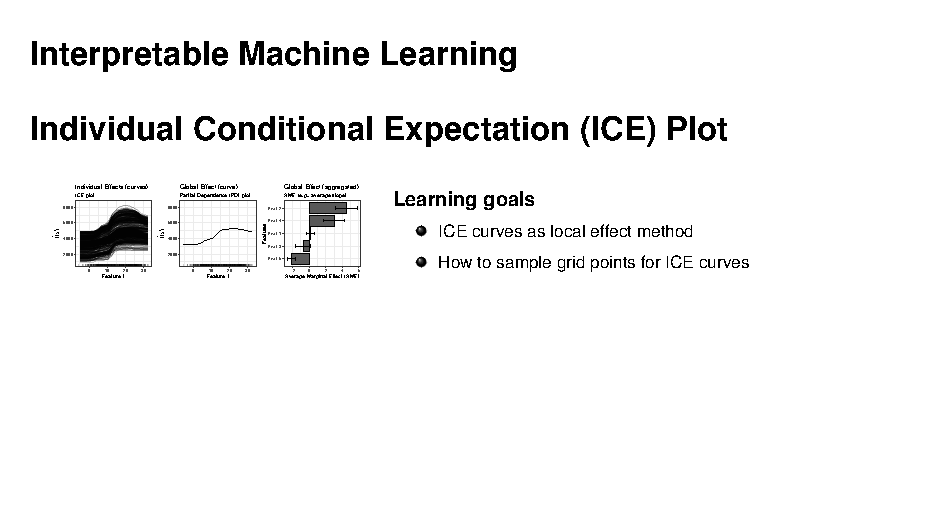
\includepdf[pages={1-last}]{slides02-fe-ice.pdf}
%\section{Feature Effects - PD plots}
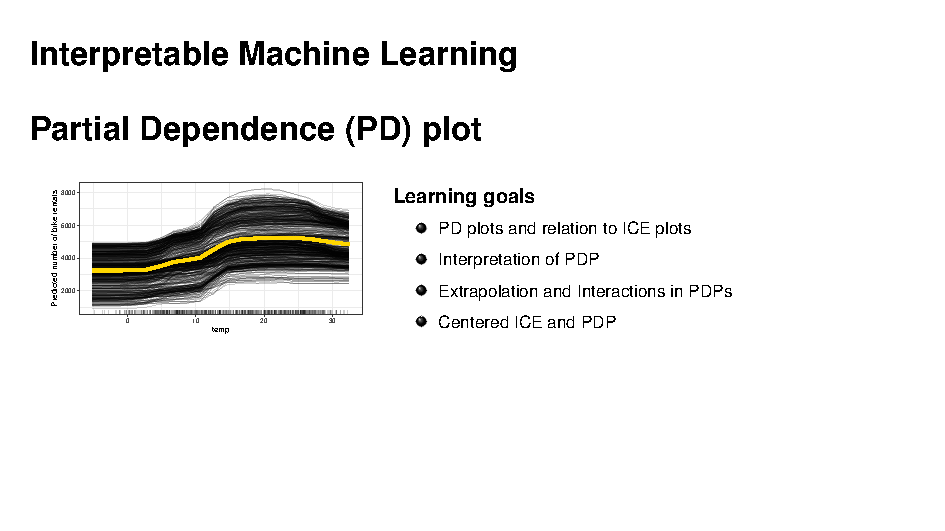
\includepdf[pages={1-last}]{slides03-fe-pdp.pdf}
\includepdf[pages={2-3}]{slides04-fe-pdp-comments.pdf}
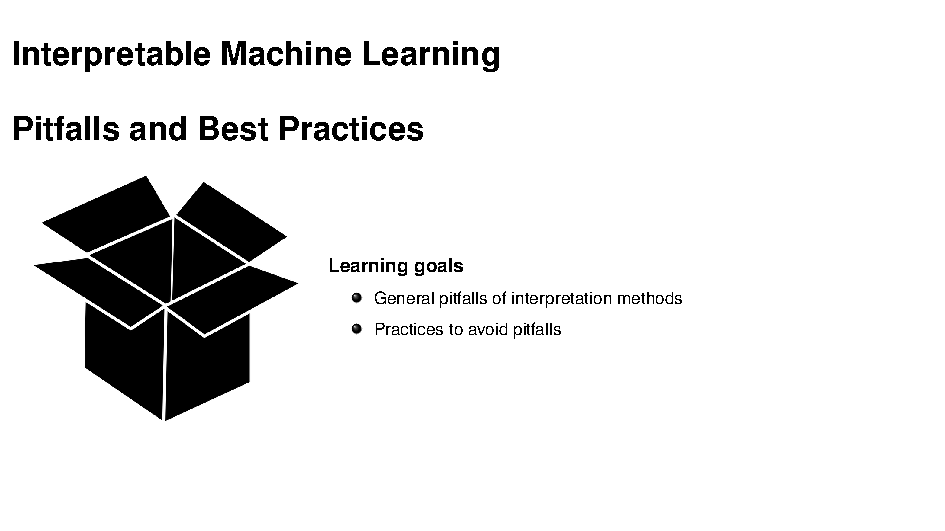
\includepdf[pages={1-8, 13-last}]{slides06-intro-pitfalls.pdf}

% \section{Feature Importance - Intro}
% \includepdf[pages={1-last}]{slides-fi-intro.pdf}

\section{Loss-based Feature Importance - PFI}
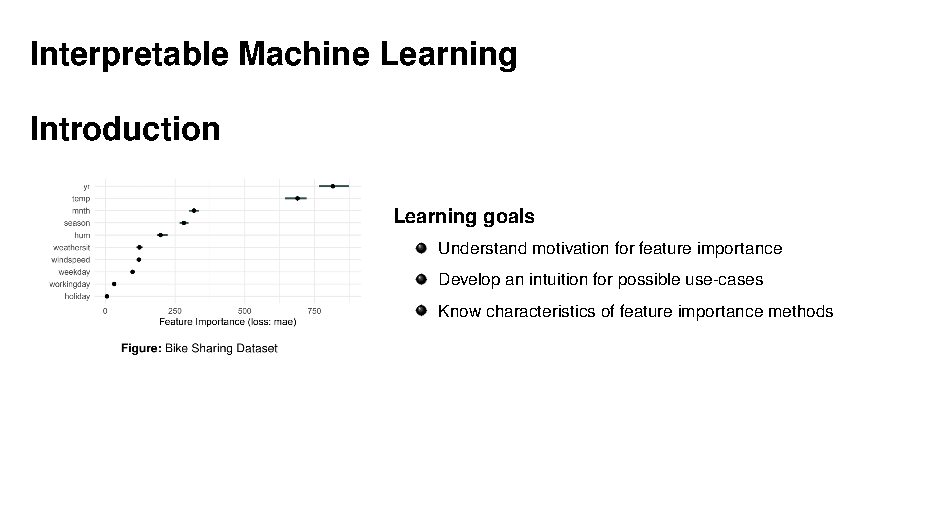
\includepdf[pages={1-7, 9-10, 12-13, 15-last}]{slides01-fi-intro.pdf}
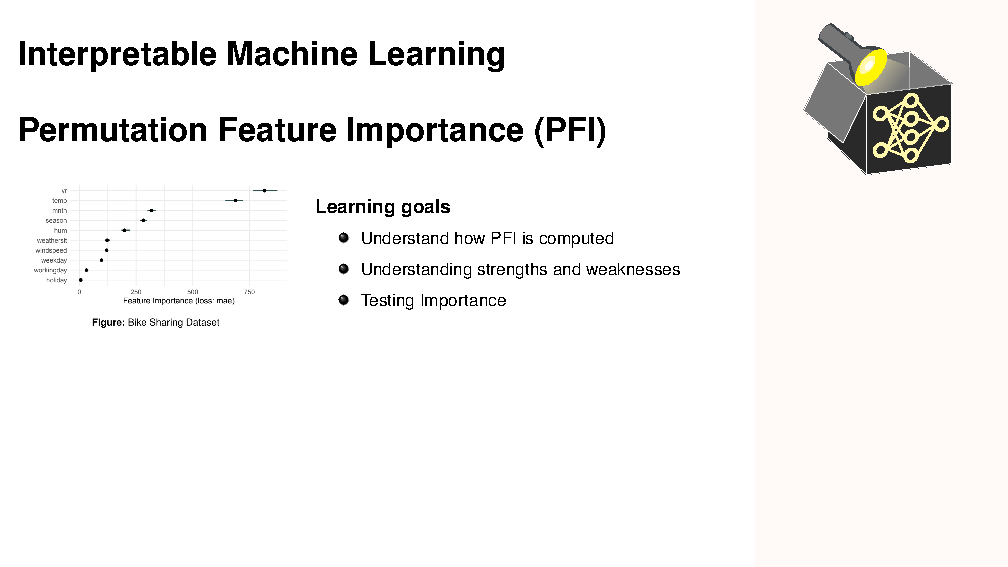
\includepdf[pages={1-22, 27-34}]{slides02-fi-pfi.pdf}
%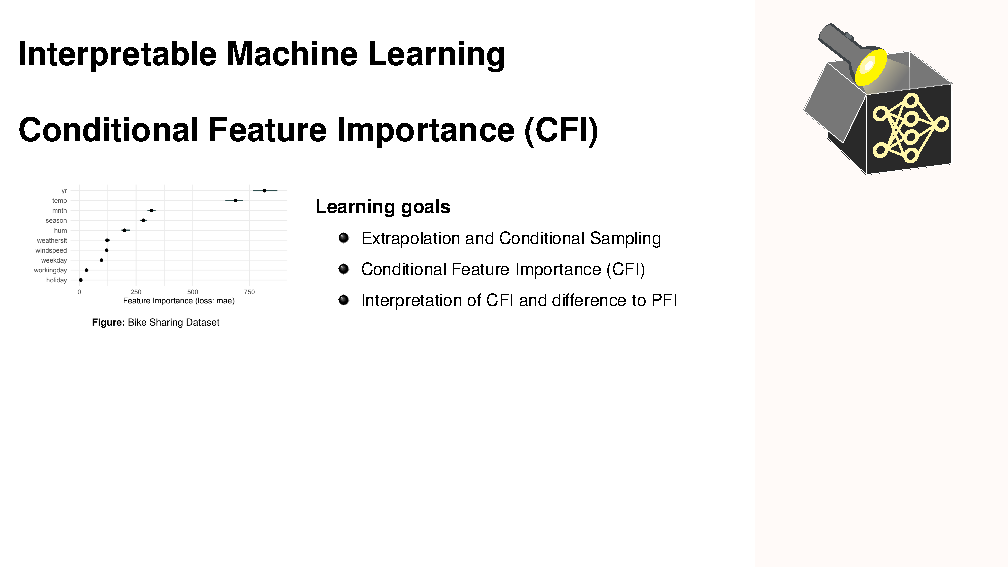
\includepdf[pages={1-7, last}]{slides03-fi-cfi.pdf}

% \section{Feature Importance - CFI}
% \includepdf[pages={1-last}]{slides-fi-cfi.pdf}
% 
% \section{Feature Importance - LOCO}
% \includepdf[pages={1-last}]{slides-fi-loco.pdf}
% 
%\section{Shapley Values - Game Theory}
%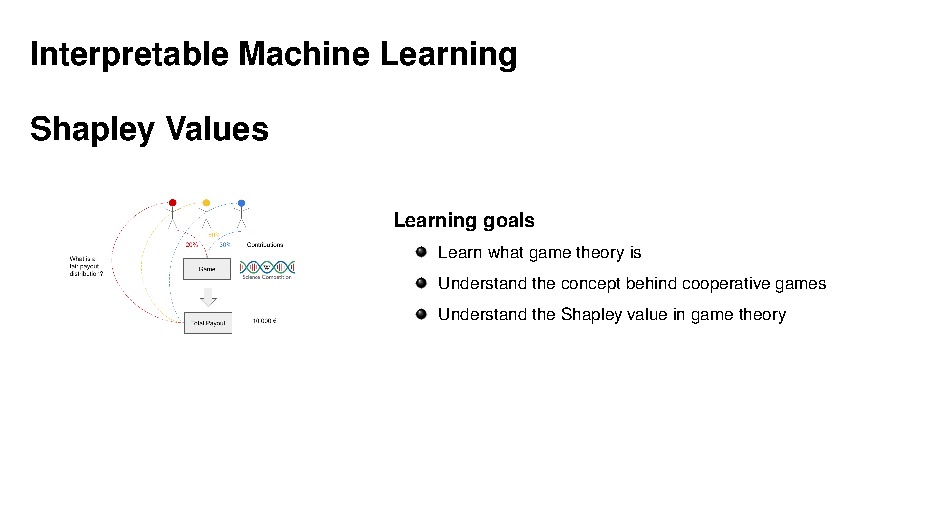
\includepdf[pages={1-last}]{slides01-shapley-game-theory.pdf}
% 
% 
% \section{Shapley Values - Global Feature Importance with SAGE}
% \includepdf[pages={1-18}]{slides-fi-sage.pdf}
% 
% \section{Shapley Values - Global Feature Importance with SAGE (Implications \& Axioms)}
% \includepdf[pages={19-last}]{slides-fi-sage.pdf}
% 
%\section{Shapley Values - Local Feature Effects}
%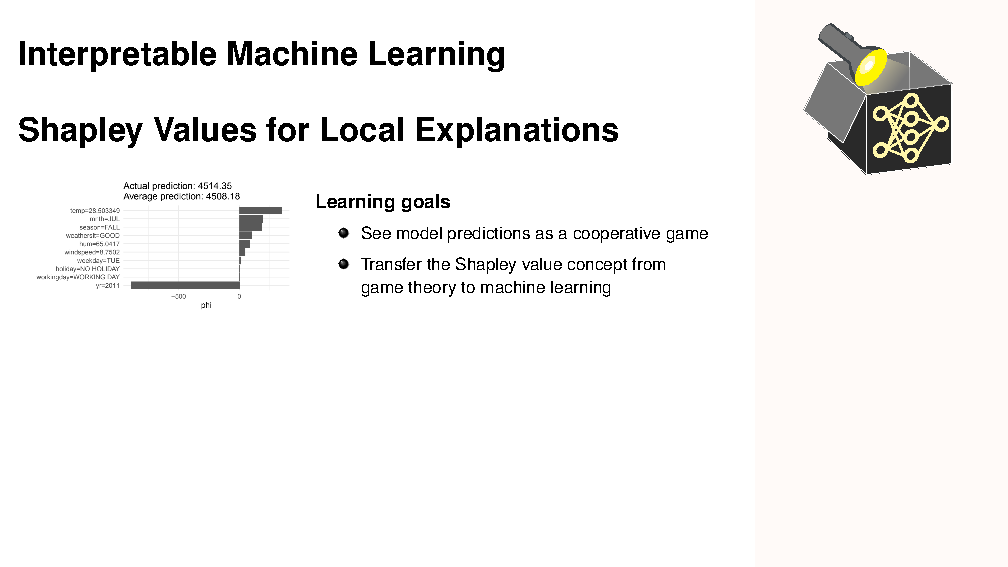
\includepdf[pages={1-last}]{slides02-shapley-ml.pdf}
% 
% \section{Optional: Shapley Values - Local Feature Effects with SHAP}
% \includepdf[pages={1-23}]{slides-shap.pdf}
% 
%\section{Optional: Shapley Values - Global Feature Effects with SHAP}
%\includepdf[pages={1-last}]{slides05-shap_global.pdf}
% 

% \section{Local Explanations - Intro}
% \includepdf[pages={9-15}]{slides-le-intro.pdf}
% 
\section{Local Explanations - LIME}
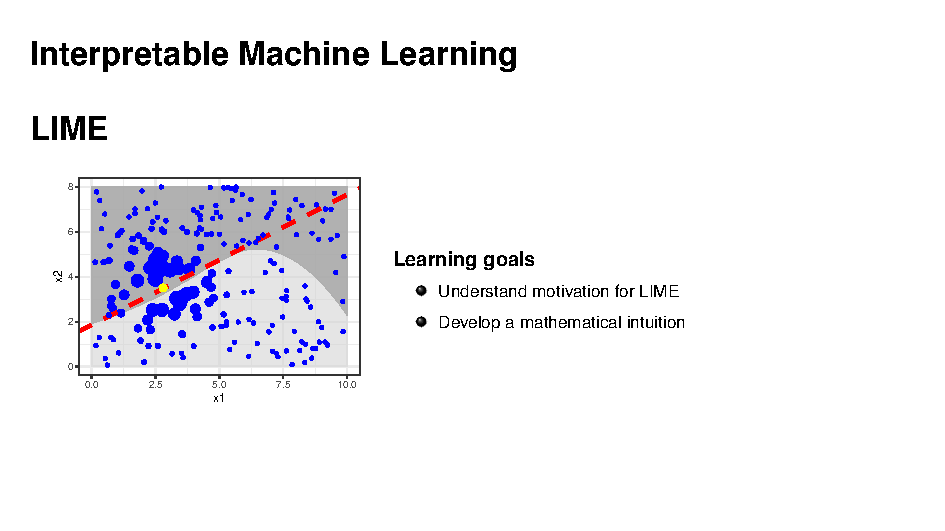
\includepdf[pages={1-last}]{slides04-le-lime.pdf}
% %\section{Local Explanations - Examples}
\includepdf[pages={2-4}]{slides05-le-lime-examples.pdf}
% 
% \section{Local Explanations - LIME Pitfalls}
% \includepdf[pages={1-last}]{slides-le-lime-pitfalls.pdf}


\section{Local Explanations - Counterfactuals}
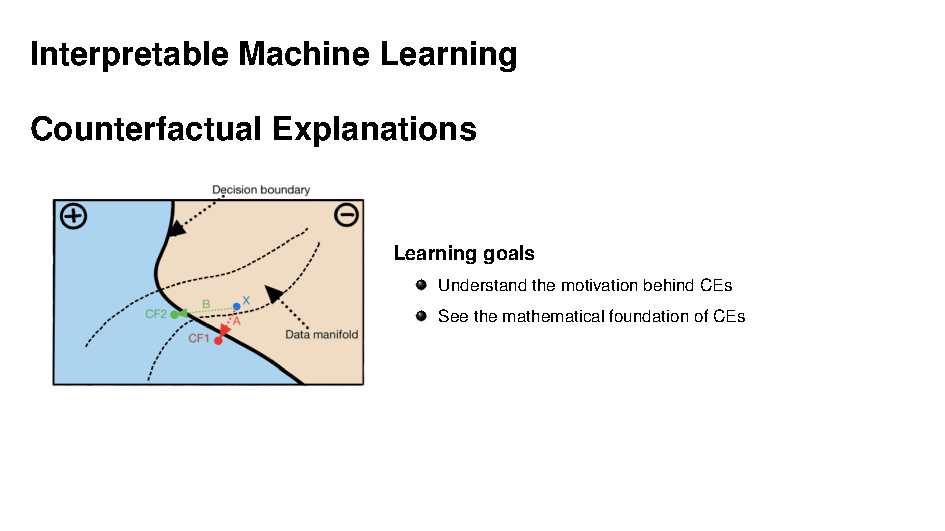
\includepdf[pages={1-3,8,13,22-last}]{slides07-le-counterfactuals.pdf}
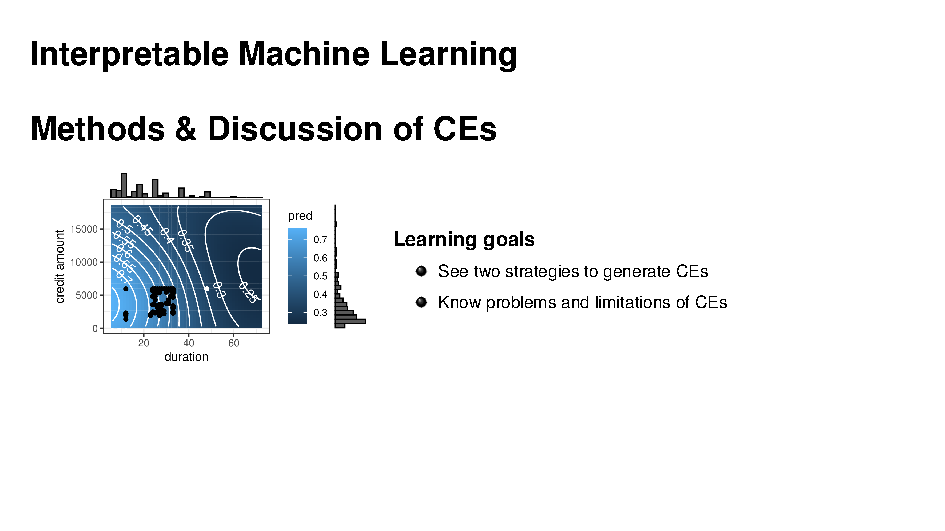
\includepdf[pages={1, 9-10, 14-21}]{slides08-le-counterfactuals-methods.pdf}


% \section{Interpretable Models}
% \includepdf[pages={1-2, 7, 14-last}]{slides-im-motivation.pdf}

\end{document}
